\section{Introduction}
\label{sec-introduction}

% introduce LPL asynchronous duty cycle media access
Smartphones have become a necessity in our lives, as we are checking our mobile phones constantly throughout the day. As a result, some privacy concerns have arisen about nearby parties peeking at our screen, namely ``shoulder surfing''. 
Given that the attacker is not malicious and merely takes several peeks out of curiosity, most works in this area are built on a threat model of an attacker observing with naked eyes, avoiding the severe data leakage effectively~\cite{eiband2017understanding}. For example, a mere stranger can hardly do any harm reading a fragment of the correspondence or acquiring the password shown on screen without any equipment.

% It is however the rare but malicious attacker, with certain familiarity and knowledge of the victim, that can do the most harm. The attacker can even be our closest friends or family members, as there are various cases in China where a child obtains Alipay password of their parents and is unaware that electronic payments consists of 'real' money, resulting in spending them lavishly in their games. Besides, specially designed equipment are not a necessity for the shoulder surfing attack. 

The privacy concerns however have been exacerbated with the rapidly developed mobile camera module these years. Equipped with multiple cameras, the newest generation of smartphones can perform 100$\times$ zooming compared to the standard 5$\times$ of single camera phones. Hardware improvements in memory also allows the burst mode at tremendous frame rates and even high-speed photography, delivering videos with thousands of frames per second. Given the commercial smartphone, the attacker can record the information reliably for propagating. And more images mean more recorded information of the victim. For example, in a Senate hearing, the Justice Secretary of Philippines, Vitaliano Aguirre II, suffered a leakage of his text messages, as someone had taken a snapshot of his smartphone \cite{Polotiko2017leakage}. To gain vital data more stealthily and accurately from even further away, the processing technique of multi-frame super resolution (SR) algorithms can be further employed by the attacker, delivering a long-range shoulder surfing threat model.

% In this present era where the leakage of a password and the disclosure of correspondence of public figures can cause great damage to the victim, we believe that it's imminent to recall attention on this new privacy threat and propose the corresponding standard of screen protection based on modern circumstances.

Unfortunately, none of existing work can mitigate this new threat model. Specifically, massive efforts have been made, from physical privacy films to alternative password entry interfaces~\cite{wiedenbeck2006design,papadopoulos2017illusionpin} and input methods~\cite{kumar2007reducing}. All of these methods however require the additional deployment cost \cite{Chun2019Keep} and cannot be widely deployed for critical privacy stages (e.g., password entry) of most scenarios. Furthermore, none of existing works can deal with the presence of developed smartphone cameras and SR algorithms in shoulder surfing scenarios. Given the ubiquitous usages of smartphones and serious damages of the data disclosure for the victim, it is imminent to recall attention on this new threat model and propose corresponding countermeasure for modern circumstances.

\begin{figure}
	\centering
	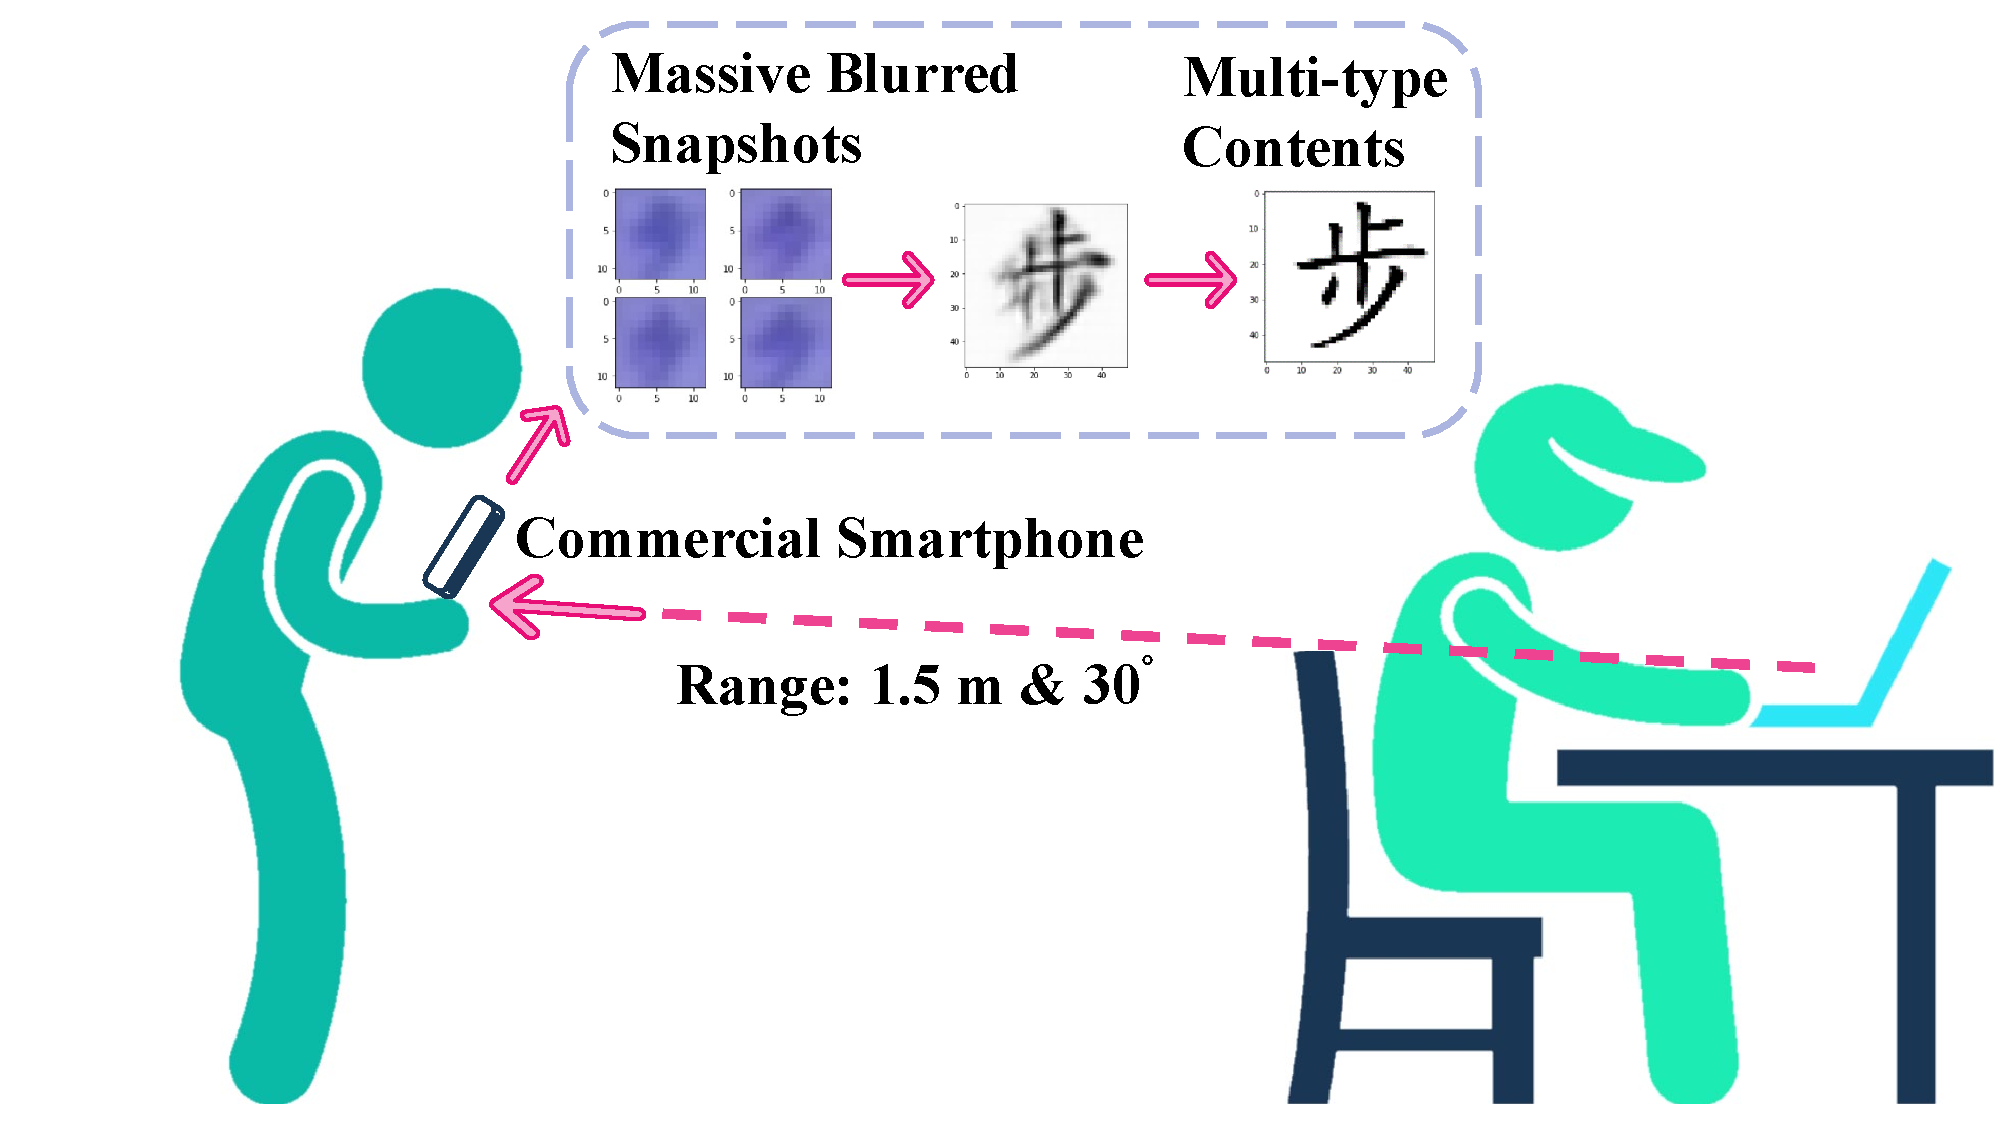
\includegraphics[width=0.48\textwidth]{pic/illustration.pdf}
    \caption{Illustration of the long-range shoulder surfing threat model on smartphones, exacerbated by the SR algorithm.}
	\label{illustration_of_system}
\end{figure}

\vspace{1mm}
\noindent
\textbf{Threat Model.} We present \textsf{SRPeek}, an end-to-end system of shoulder surfing using the SR algorithm, illustrated in Figure~\ref{illustration_of_system}. 
While the victim's reading private information in public, the attacker, standing within 1.8 meters behind him, raises his commercial smartphone and zooms in on the victim's screen. Then he can take 10 to 20 snapshots rapidly in burst mode (about 10 frames per second), and process them with a multi-frame SR technique to generate a high-resolution result. The whole process only takes a few seconds and can even be repeated at a 2 second interval, enabling the attacker to monitor the victim's screen continuously, not missing any detail. Meanwhile, few people would suspect a stranger holding his smartphone at 1.8 meters behind them. Given the newest generation of smartphones equipped with telephoto lenses and capable of optical zooming, this distance can reach a staggering 6 meters, posing a silent but deadly threat to screen privacy.

\vspace{1mm}
\noindent
\textbf{Challenges.} Creating a powerful SR based shoulder surfing threat model, however, is not trivial, especially for commercial smartphones in real time. And we achieve \textsf{SRPeek} by overcoming four key challenges.

\begin{itemize}[leftmargin=*]
  \item \textbf{Blurriness of input images.} The most prominent one is the blurriness of captured snapshots, as they are taken secretly and hurriedly at extreme range, without specially focusing. It can be further exacerbated by straining the magnification of the smartphone lenses. Unlike most SR applications and datasets working with ``normally'' captured snapshots (e.g., scenery, scanned images) \cite{nasrollahi2020deep,lyn2020image}, these snapshots exhibit lower concentrations of information and more artifacts as Figure~\ref{illustration_of_system} shows, requiring a reliable ``reconstruction'' than ``interpolation''. Since blurrier input means less information, rendering a greater possibility of reconstructing the wrong character. 
  % In deep learning based methods, a deep network often leads to gradual divergence from the truth as the data is propagated deeper through the network pipeline, resulting in 'fake' high-resolution images, especially when the subjects are the discrete strokes of characters, instead of details and texture of everyday objects. As a matter of fact, most works on multi-frame SR function on video clips \cite{lucas2019generative} or multiple snapshots \cite{wronski2019handheld}, however, our application is subtly different from the two. 
  On one hand, each snapshot is blurred with a randomly different PSF kernel, removing the consistency between neighboring frames. Thus it cannot be approximated as video clips using a constant, isotropic gaussian kernel; on the other hand, each defocused snapshot only contains fractions of information, analogous to pieces of a jigsaw puzzle. Thus it poses a greater demand for integration abilities of the SR algorithms than most other SR applications.
  % and the only chance of recovering the ground truth is to compare each photo against others. 
%  Few useful information can be extracted separately and merged directly to produce perceptible results if processed by common procedures to enhance the resolution of blurred snapshots\cl{citation?}. 
  \item \textbf{Super resolution with multiple snapshots.} To resolve the blurriness of input snapshots, a SR algorithm on a smartphone is required to recover the blurred contents. However, none of existing SR algorithms can be adapted for this attack scenario, especially with massive extremely blurred snapshots as input. Since smartphones can capture 10 snapshots per second in burst mode. Specifically, the difference between videos and multiple snapshots rules out existing image/video super resolution algorithms~\cite{lucas2019generative,kappeler2016video}. The reason has two folds. First, massive input leads to the increase in model complexity, making it unsuitable for mobile deployment. Second, the nature of our task requires to do pixel-wise correlation and comparison in the same coordinate with consecutive snapshots throughout our construction process. Otherwise we cannot tell if, for example, it is one stroke or two parallel strokes that is shown in these two darker pixels on this snapshot.
  \item \textbf{Model complexity and variable input.} We have to operate our threat model locally on commercial smartphones in a real-time manner rather than remotely in cloud server. Since 1) the latter requires a stable internet access, and 2) sending multiple snapshots across the Internet will consume time and bandwidth. Given the required 10 to 20 snapshots to be processed for the ideal content recovery, we have 1-2 seconds as the minimum interval between each output frame, rendering a limited period for calculation with the restricted power and RAM. In case where the display on the target screen changes more frequently, fewer snapshots and less processing time are available for each scene. Consequently, it cannot only require a more precise network model, but also a model that can deal with dynamic inputs efficiently, either 3 or 20 snapshots.
  \item \textbf{Complexities of characters.} To deploy our threat model broadly for real-life scenarios (e.g., record passwords or e-mails), it is supposed to reconstruct complex characters with multiple strokes, such as Chinese characters shown in Figure~\ref{illustration_of_system}. Composed of multiple strokes, characters are distributed discretely in the pixel-wise snapshot and different with other entities (e.g., faces and natural objects), rendering unique challenges. In some cases, messing up a stroke even slightly can shorten or lengthen a stroke, leading to a different character for misunderstandings. Unlike most SR applications working on similarity between their output and the ground truth, our network architecture and training process must be engineered to recover readable contents. Another challenge is the imbalanced element for words. Since we know certain stroke or alphabet of Chinese and English characters can occur more frequently, results in lower prediction accuracy over the less common, unconventionality shaped characters.
\end{itemize}

\vspace{1mm}
\noindent
\textbf{Summary of Evaluation Results.}
Equipped with our uniquely designed SR algorithm, our system can help the attacker read the characters shown on the victim's screen with above 90\% accuracy at 1.8m distance on a smartphone without optical zooming, or 6m on a phone with optical zooming in our experimental settings. \textsf{SRPeek} can capture snapshots and produce high-resolution images constantly with about 2 seconds interval. Our experiments in real life scenarios show that it can decipher texts or passwords of the victim at a safe distance, without alarming the victim, posing a serious threat to screen privacy.

\vspace{1mm}
\noindent
\textbf{Contributions.} This paper makes the following contributions:
\begin{itemize}[leftmargin=*]
  \item	We propose \textsf{SRPeek}, an end-to-end threat model of shoulder surfing from a broad range, which can be deployed on commercial smartphones. To the best of our knowledge, we are the first to consider the presence of smartphone cameras and SR algorithms in shoulder surfing scenarios.
  \item	We design a multi-frame SR neural network architecture to reconstruct massive extremely blurred and defocused snapshots. It can be further extended to other text-recognition applications.
  \item	We evaluate this new shoulder surfing threat model in multiple scenarios. And it outperforms the state-of-the-arts for content recognition, calling for the new privacy concern.
\end{itemize}
% describe the organization of the paper

\vspace{1mm}
The rest of the paper is organized as follows. Section~\ref{sec-related-work} describes the related work, especially the state-of-the-arts for the shoulder surfing and SR techniques. We present the system and network design in Section~\ref{sec-design}, followed by the implementation and evaluation in Section~\ref{sec-implementation-and-training} and~\ref{sec-evaluation}. We further wrap up this paper by delivering the limitations and countermeasures of our system in Section~\ref{sec-limitations-and-discussions}. And the conclusion is shown in Section~\ref{sec-conclusion}.
